\chapter{背景:音楽}

本章では、本論文での音の定義を行った後に、音楽の特徴量抽出の方法を紹介する。

\section{音の定義}

音とは、弾性体中を伝播する弾性波により起こされる音波が聴覚により感じられるもののことである。また、音は騒音と楽音の大きく二つに分けることができる。騒音とは不規則な振動の音波による音のことであり、楽音とは周期生のある音波による音のことである。本論文では、楽音のことを音と呼ぶ。

音は長さ、大きさ、高さ、音色の四要素から成り立ち、人間はこれらの要素を知覚することができる。また、図\ref{fig:gakuon}は音の四要素について簡単に示した図である。

\begin{figure}[b]
\begin{center}
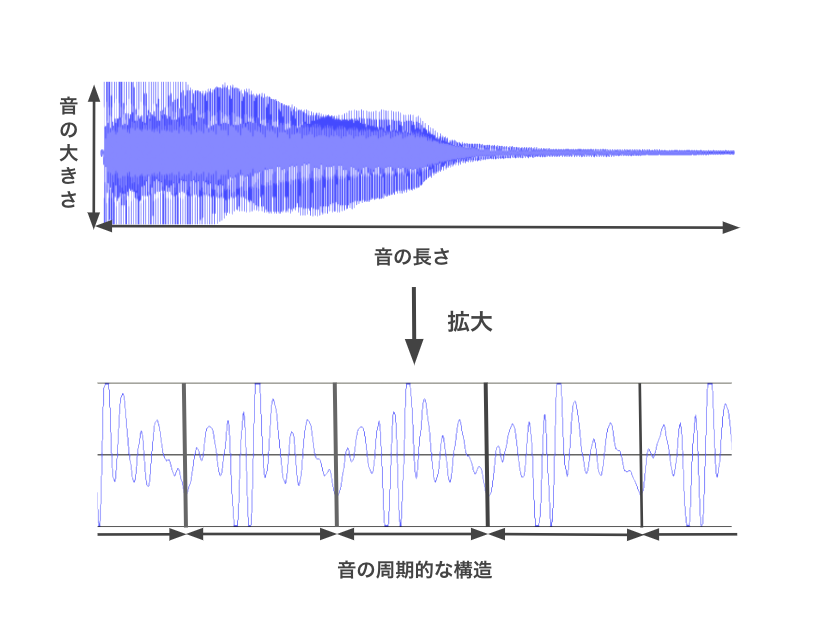
\includegraphics[width=0.6\hsize]{figure/gakuon.png}
\caption{音の四要素}
\label{fig:gakuon}
\end{center}
\end{figure}

\subsection{音の長さ}

音の長さは図\ref{fig:gakuon}のように音波の時間の長さにより決まる。一般に、音の長さは楽譜上での時間の長さ~(音価)~により決まるが、本論文では音波の時間の長さにより決まるものとする。

\subsection{音の大きさ}

音の大きさは図\ref{fig:gakuon}のように音波の振幅により決まる。また、人間には振幅の大きい音は大きく、振幅の小さい音は小さく知覚される。

\subsection{音の高さ}

音の高さは音波の周波数により決まる。つまり、図\ref{fig:gakuon}のような音の周期的な構造の長さにより決まる。また、人間には周波数の高い音は高く、周波数の低い音は低く知覚さる。そして、複数の周波数の音波が音に含まれる場合は最も低い周波数成分の音波~(基音)~を音の高さとして知覚する。

国際の音名表記では、C,D,E,F,G,A,Bのセットを西洋音楽の七音音階におけるオクターブとして定める。さらに、それぞれのオクターブに番号を振り、440~Hzの音をA4と定めることで、任意の半音の絶対的な表記を可能にしている。また、国際の音名表記では半音よりさらに細かい音~(微分音)~を表すことはできないが、本論文では扱わない。

\subsection{音の音色}

音の長さと高さと大きさが同じであっても異なった音として人間には知覚されることがある。この違いを音色と呼ぶ。また、音色は図\ref{fig:gakuon}のような音の周期的な構造の形により決まる。

\begin{figure}[b]
\begin{center}
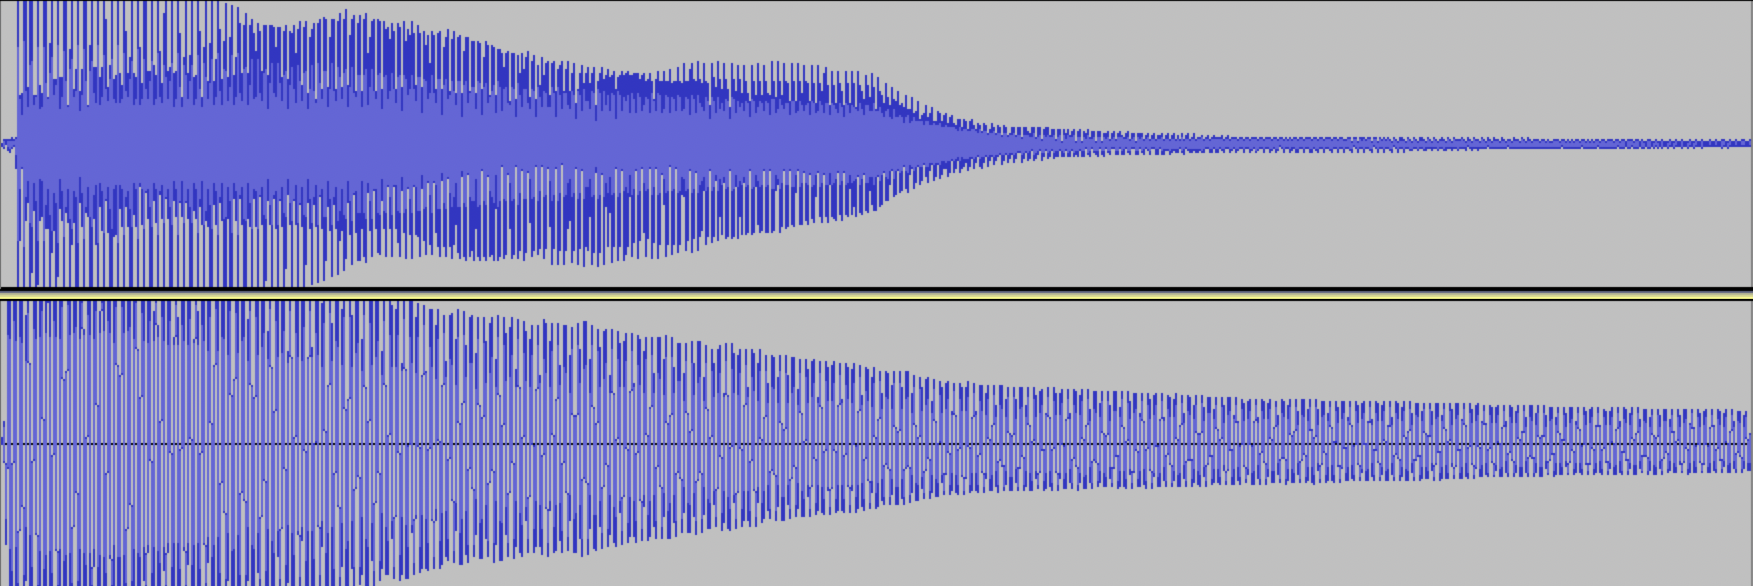
\includegraphics[width=\hsize]{figure/c4_guitar_harp.png}
\caption{ギターとハープの音色}
\label{fig:guitar_harp_comp}
\end{center}
\end{figure}

ここで、長さと高さと大きさが同じギターとハープの音波を図\ref{fig:guitar_harp_comp}に示す。これらの音は波形が異なるので、その音色も異なる。また、音色の異なる音どうしは基音よりも高い音~(上音)~の組み合わせが異なるため、このような波形の違いが生まれる。

\section{音楽の特徴}

%以下の自分の考えと融合させる
\begin{comment}
\section{展望}

一般に、音楽で特定の音色への変換を行うことは難しいが、次の三つの要素に分解することで単音での音色の変換を音楽へと適用することが可能であると考えられる。また、三つの要素とは、楽器の重ね合わせ、音の重ね合わせ、時間方向の音の繋ぎ方であり、それぞれについて具体的に以下で説明をする。

\subsection{楽器の重ね合わせ}
    
音楽はそれぞれの楽器により奏でられた音の重ね合わせになっている。楽器ごとに音色は異なるので楽器ごとの音波に分解して音色変換を行う~(音源分離)~が必要であると考えられる。なお、楽曲の作成時に楽器ごとに分離したデータ~(パラデータ)~で保存しておけば、音源分離を行わずに直接楽器ごとの音波を利用できる。

\subsection{音の重ね合わせ}

ある単位時間の音に注目した時、楽器ごとの音波に分解してもその単位時間で異なった高さや大きさの音の重ね合わせになっていることがある。この場合は、今回の提案手法で用意したデータセット以外に和音のデータセットも加えて学習させることで表現可能であると考えられる。

\subsection{音の繋ぎ方}

%他の工夫があるかも

楽器ごとの音波に分解し単位時間の音が表現できた時、時間方向に音を繋ぐ必要がある。時間方向については先程定めた単位時間で区切って順に変換していくことで可能であると 考えている。また、区切るのみでの変換が難しい場合は自己回帰モデルを取り入れるなどの工夫が必要であると考えている。
\end{comment}

音楽をニューラルネットワークにて扱う場合、音楽特有の特徴量抽出が必要である。また、音楽の特徴には、主観的な問題とタイムスケールの問題がある。

\subsection{音楽の主観性}

まず、主観性について。例えば、音楽のジャンルの分け方はかなり主観に依存する。それに対し、ピッチやテンポは主観性が弱い(が、曖昧でもある)。ディープラーニングはこれらの二つの問題に対してある程度対応できている。主観さの裏にある論理を解明しない限りは、人間の手で特徴量を設定するのは難しい。従って、データ駆動でend-to-endな学習を利用することができる。さらに、新たな洞察を得ることもできる。例えば、異なる音楽間の関係性。また、よく知られた論理があればネットワーク構築にも役立つ。

\subsection{音楽の時間方向のスケール}

次にタイムスケールについて、考慮すべき時間のスケール。例えば、テンポや音の高さは音楽全体では変化するものの短い時間で見れば静的である。このような場合は時間のスケールは長いと言える(時間不変性の問題)。それに対し、音色は短いスケールのタイムフレームであっても変わりうる。従って、このような場合は時間のスケールは短い(時間可変性の問題)。

このように、それぞれの特徴が異なった主観性やタイムスケールを持つので、対処法が変わってしまう。

\section{音楽の表現}
\label{sec:preprocess}

ニューラルネットワークで扱うために音の表現を工夫する必要がある。ニューラルネットワークの学習を行う場合は音楽を音響信号としてサンプリングした際の一次元データではなく、何らかの加工を施した二次元データを用いることが多い。また、この二次元の軸はほとんどの場合でも時間と周波数である。

また、音楽の表現を用いる際にはそれぞれがどのような特徴を持っているのかを把握する必要がある。また、例えばDNNは計算負荷のかかる手法なので、それぞれの段階で最適化が必要となる。最適化の一つとしては、入力のデータを変換することである。この変換により、ネットワークが音楽の情報を効果的に利用することができ、効率化できる(メモリの利用量を軽くし、計算を軽くすることができる)。

多くの場合は二次元の表現は効果的なデータとして提供する。信号を異なる周波数成分に分解することにより、信号の情報が明確化される。さらに、二次元の場合は画像と同じアプローチを使うことができるが、異なる点ももちろん存在する。まず、画像の場合は色合いなどが局所的に相互に関係しあう。それに対し、例えばスペクトログラムの場合は、周波数成分の方向では相互にハーモニックに関係し合うものの、局所的な相互関係は弱い。ハーモニックな関係を把握するために表現を変更するような研究もある。また、物体認識ではスケール不変性も求められるが、音楽についてはあまり関係ない

\subsection{音響信号}

音響信号は最も素朴な表現であり、他の表現は全て一度音響信号を経由して変換されたものである。音そのものはアナログ信号であるが、デジタル信号である音響信号へと変換される。また、音響信号はそれぞれの単位時間で量子化が行われる。また、音響信号をニューラルネットワークを通して学習に用いるには、より多くのデータセットを用いた特徴量の把握が必要であると考えられ、多くの研究では二次元の表現が好まれてきた。ただ、最近でも1次元での畳み込みは時間周波数の変換でよく用いられる。←なんで?、自分の読んだ既存研究も

% 以降はちゃんと勉強したら詳しく書く
%とりあえず訳す

\subsection{STFT}

時間と周波数で表す二次元の音の表現として代表的かつ基本的なものがSTFTである。

\subsection{メルスペクトログラム}

\subsection{CQT}

\subsection{クロマグラム}

\subsection{DDSP}

%音声処理勉強してここに載せる(大幅な改変)
%いいやつを見つけた

%以下の流れ

%まず基本的なこと

%既存研究でもこんな感じ

%それぞれに特徴があるけど…

\begin{comment}
本章では、主要な音声処理の方法を紹介する。

以下の単語は説明

サンプリング周波数] デジタル信号の1秒あたりの標本化の回数

サンプリング数] 音波のデジタル信号の標本化の合計の回数のこと

量子化ビット数] デジタル信号の細かさを表現するビット数のこと

チャンネル数] モノラルな音声出力の総数のこと

%短期vs長期
%長期は生成しておいて短期は後から
%音楽の研究の例はをどこかに
既存研究の軽い紹介…。GAN,Pix2pix…。音楽の変換の研究(Hukebox,スペクトログラム,MIDI)…。この手法では…。音色の変換のみを扱うことで短期的な構造のみに着目できる点で他の音楽生成の研究よりも計算時間を削減できると期待される。
\end{comment}